% ============================================================================
% Artigo do projeto da disciplina Aplicações de DSP (ADSP) - PUCRS
% Formato: modelo "Formato_Projeto_ADSP" (duas colunas, carta, Times)
%   - margens: 20 mm em cima/embaixo, 18 mm nas laterais; 6 mm entre colunas
%   - recuo de parágrafo de 3.5 mm; sem numeração de páginas; máximo 6 páginas
%   - título 14 pt negrito; autores 12 pt; afiliação e texto 10 pt;
%     resumo 9 pt negrito; e-mail 9 pt itálico; legendas e notas 8 pt
% Compilar com pdflatex (duas vezes, por causa das referências cruzadas).
% ============================================================================
\documentclass[10pt,twocolumn,letterpaper]{article}

\usepackage[utf8]{inputenc}
\usepackage[T1]{fontenc}
\IfFileExists{brazil.ldf}{\usepackage[brazil]{babel}}{}
\usepackage{mathptmx}                 % Times Roman (texto e equações)
\usepackage[letterpaper,top=20mm,bottom=20mm,left=18mm,right=18mm,columnsep=6mm]{geometry}
\usepackage{amsmath}
\usepackage{graphicx}
\usepackage{booktabs}
\usepackage{array}
\usepackage{titlesec}
\usepackage[font=footnotesize,labelsep=period,justification=centering]{caption}
\usepackage{tikz}
\usetikzlibrary{positioning,arrows.meta}
\usepackage{url}
\usepackage{microtype}

\pagestyle{empty}                     % não numerar as páginas
\setlength{\parindent}{3.5mm}
\DeclareMathOperator{\med}{med}

% --- Títulos de seção no estilo do modelo -----------------------------------
% I. INTRODUÇÃO (centralizado, maiúsculas, 10 pt, sem negrito)
\renewcommand{\thesection}{\Roman{section}}
\titleformat{\section}{\centering\normalsize}{\thesection.}{0.4em}{\MakeUppercase}
\titlespacing*{\section}{0pt}{12pt plus 2pt}{8pt}
% A. Subtítulo (itálico, à esquerda)
\renewcommand{\thesubsection}{\Alph{subsection}}
\titleformat{\subsection}{\normalsize\itshape}{\thesubsection.}{0.4em}{}
\titlespacing*{\subsection}{0pt}{8pt plus 2pt}{5pt}
% 1) Subtítulo: (itálico, na mesma linha do texto)
\renewcommand{\thesubsubsection}{\arabic{subsubsection}}
\titleformat{\subsubsection}[runin]{\normalsize\itshape}{\thesubsubsection)}{0.4em}{}[:]
\titlespacing*{\subsubsection}{\parindent}{2pt}{0.5em}

% --- Legendas: "Fig. 1." embaixo e "TABELA I" em cima, em 8 pt ----------------
\captionsetup[figure]{name=Fig.}
\DeclareCaptionLabelFormat{tabmodelo}{\MakeUppercase{#1}~#2}
\DeclareCaptionFormat{tabmodelo}{#1\\\MakeUppercase{#3}}
\captionsetup[table]{name=Tabela,labelformat=tabmodelo,format=tabmodelo,
                     font=footnotesize,skip=4pt}
\renewcommand{\thetable}{\Roman{table}}
\renewcommand{\figurename}{Fig.}
\renewcommand{\tablename}{Tabela}

% Referências no formato do modelo, título "REFERÊNCIAS" numerado como seção
\makeatletter
\renewcommand\@biblabel[1]{[#1]}
\renewenvironment{thebibliography}[1]
  {\section{Referências}\footnotesize
   \list{\@biblabel{\@arabic\c@enumiv}}%
        {\settowidth\labelwidth{\@biblabel{#1}}\leftmargin\labelwidth
         \advance\leftmargin\labelsep\usecounter{enumiv}%
         \let\p@enumiv\@empty\renewcommand\theenumiv{\@arabic\c@enumiv}%
         \itemsep 2pt}%
   \sloppy\sfcode`\.\@m}
  {\endlist}
\makeatother

\begin{document}

% ============================================================================
% TÍTULO E AUTORES
% ============================================================================
\twocolumn[{%
\begin{center}
  {\fontsize{14}{17}\selectfont\bfseries
   Leitura Automática de Displays de Multímetros por Visão Computacional\\
   para Apoio à Calibração\par}
  \vspace{16pt}
  \begin{tabular}{@{}c@{\hspace{30mm}}c@{}}
    {\fontsize{12}{14}\selectfont Arthur Mazot} &
    {\fontsize{12}{14}\selectfont Sophia Mendes} \\[2pt]
    Escola Politécnica & Escola Politécnica \\
    Pontifícia Universidade Católica do RS & Pontifícia Universidade Católica do RS \\
    Av. Ipiranga, 6681 & Av. Ipiranga, 6681 \\
    Porto Alegre, RS, 90619-900 & Porto Alegre, RS, 90619-900 \\
    BRASIL & BRASIL \\
    {\fontsize{9}{11}\selectfont\itshape arthur.mazot@edu.pucrs.br} &
    {\fontsize{9}{11}\selectfont\itshape sophia.mendes@edu.pucrs.br}
  \end{tabular}
\end{center}
\vspace{14pt}
}]

% ============================================================================
% RESUMO
% ============================================================================
{\fontsize{9}{11}\selectfont\bfseries
\noindent\textit{Resumo} -- Este trabalho apresenta um sistema para a leitura
automática do display de sete segmentos de multímetros digitais durante
procedimentos de calibração, a partir das imagens de uma webcam. O operador
seleciona a região do display, e o sistema extrai o recorte como a mediana de
oito quadros consecutivos, avalia a qualidade da imagem (luminosidade,
contraste, reflexos e nitidez), envia o recorte a um modelo de reconhecimento
e valida o valor lido com um conjunto de alertas: leitura vazia, salto brusco,
mudança de casas decimais, câmera movida e valor fora da faixa esperada. Cada
leitura é classificada como válida, duvidosa ou falha e registrada num arquivo
CSV, junto com o recorte usado. O sistema foi implementado em Python, com
OpenCV e uma interface em Tkinter organizada em três etapas: visualização,
configuração e captura.\footnote{Trabalho final da disciplina Aplicações de
DSP, Escola Politécnica, PUCRS, 2026.}\par}

% ============================================================================
\section{Introdução}
% ============================================================================

Na calibração de multímetros, o instrumento sob teste é submetido a uma
sequência de valores conhecidos (pontos de calibração), e a indicação do seu
display é comparada ao valor de referência. Em muitos laboratórios essa
indicação ainda é lida e anotada por um operador, o que torna o processo lento,
cansativo e sujeito a erros de transcrição, principalmente quando cada ponto
exige várias leituras repetidas ou quando o ensaio se estende por vários ciclos.

Grande parte dos multímetros de bancada e portáteis não possui interface de
comunicação, ou possui uma interface proprietária. A alternativa mais geral é
ler o próprio display, como faria o operador. Displays de cristal líquido (LCD)
de sete segmentos, porém, apresentam dificuldades para a visão computacional:
baixo contraste entre segmentos e fundo, reflexos da iluminação do ambiente e
de LEDs próximos, cintilação e variação da quantidade de dígitos, do ponto
decimal e dos símbolos de unidade entre modelos.

Este trabalho descreve um sistema que automatiza essa leitura com uma webcam
comum. A ênfase está no processamento de sinais aplicado à imagem: a redução de
ruído por mediana temporal, as métricas usadas para decidir se a imagem tem
qualidade suficiente para ser lida, a detecção de deslocamento da câmera por
correlação normalizada e a validação do valor lido ao longo do tempo. O
reconhecimento dos dígitos em si é feito por um modelo treinado, executado na
plataforma Roboflow \cite{roboflow}.

% ============================================================================
\section{Visão Geral do Sistema}
% ============================================================================

O sistema é composto por uma webcam USB apontada para o display do multímetro e
por um computador com Windows. A câmera é configurada para 1920 × 1080 pixels
no formato MJPG e é lida por uma \textit{thread} dedicada, que mantém sempre o
quadro mais recente. Assim, a pré-visualização da interface e a captura das
leituras funcionam em paralelo, sem que uma espere pela outra.

O software foi escrito em Python 3.11, com as bibliotecas OpenCV \cite{opencv}
e NumPy para o processamento das imagens, o \textit{inference-sdk} para a
comunicação com o modelo de reconhecimento e o Tkinter para a interface. O
fluxo de trabalho foi dividido em três etapas, que correspondem às três abas da
interface:

\begin{enumerate}
  \setlength{\itemsep}{0pt}
  \item \textit{Calibração da visualização}: o operador seleciona o display com
        um retângulo sobre a imagem da câmera, e o teste de qualidade é
        executado continuamente até a imagem ser considerada adequada;
  \item \textit{Configuração da captura}: intervalo entre leituras, número de
        leituras, unidade, ponto de calibração, ciclo, faixa esperada, alertas
        por valor e arquivo de registro;
  \item \textit{Captura e acompanhamento}: as leituras são feitas no intervalo
        definido e exibidas com o seu estado e os alertas gerados.
\end{enumerate}

O processamento de cada leitura segue o diagrama da Fig.~\ref{fig:fluxo}. As
verificações de qualidade e de câmera movida são periódicas (por padrão, a
cada cinco leituras, sempre incluindo a primeira), pois o seu custo é maior que
o da leitura e as condições de captura mudam lentamente.

\begin{figure}[!t]
\centering
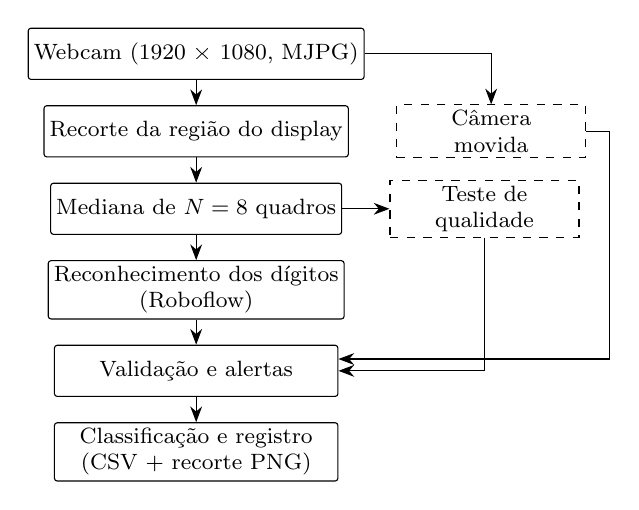
\begin{tikzpicture}[
  node distance=3.2mm,
  bloco/.style={draw, rounded corners=1pt, align=center, font=\footnotesize,
                minimum width=36mm, minimum height=6.5mm, inner sep=2pt},
  lateral/.style={draw, dashed, align=center, font=\footnotesize,
                  minimum width=24mm, minimum height=6.5mm, inner sep=2pt},
  seta/.style={-{Stealth[length=2mm]}}]
  \node[bloco] (cam) {Webcam (1920 × 1080, MJPG)};
  \node[bloco, below=of cam] (roi) {Recorte da região do display};
  \node[bloco, below=of roi] (med) {Mediana de $N = 8$ quadros};
  \node[bloco, below=of med] (lei) {Reconhecimento dos dígitos\\(Roboflow)};
  \node[bloco, below=of lei] (ale) {Validação e alertas};
  \node[bloco, below=of ale] (log) {Classificação e registro\\(CSV + recorte PNG)};
  \node[lateral, right=6mm of med] (qual) {Teste de\\qualidade};
  \node[lateral, right=6mm of roi] (mov) {Câmera\\movida};
  \draw[seta] (cam) -- (roi);
  \draw[seta] (roi) -- (med);
  \draw[seta] (med) -- (lei);
  \draw[seta] (lei) -- (ale);
  \draw[seta] (ale) -- (log);
  \draw[seta] (med) -- (qual);
  \draw[seta] (cam.east) -| (mov.north);
  \draw[seta] (qual.south) |- (ale.east);
  \draw[seta] (mov.east) -- ++(3mm,0) |- ([yshift=1.5mm]ale.east);
\end{tikzpicture}
\caption{Processamento de cada leitura. Os blocos tracejados são executados
periodicamente.}
\label{fig:fluxo}
\end{figure}

% ============================================================================
\section{Processamento da Imagem}
% ============================================================================

\subsection{Recorte e Mediana Temporal}

A região do display é definida pelo operador arrastando o mouse sobre a imagem.
O retângulo resultante $(x, y, w, h)$ é limitado às dimensões do quadro, e
seleções menores que 10 × 10 pixels são descartadas.

A cada leitura, o sistema recolhe o recorte de $N$ quadros novos (nunca reutiliza
um quadro já usado) e calcula, para cada pixel $(m, n)$ e cada canal de cor, a
mediana ao longo do tempo:
\begin{equation}
  \hat{I}(m,n) = \med\{I_1(m,n),\, I_2(m,n),\, \ldots,\, I_N(m,n)\},
  \label{eq:mediana}
\end{equation}
em que $I_k$ é o recorte do $k$-ésimo quadro e $N = 8$. A mediana é um filtro
não linear robusto a valores atípicos \cite{huang}: ela atenua o ruído do
sensor, como faria uma média, mas remove sem borrar os eventos que afetam
poucos quadros, como a cintilação da iluminação, a atualização parcial dos
segmentos do LCD e o reflexo momentâneo de um objeto em movimento. Como a cena
é estática, a filtragem no tempo não reduz a resolução espacial do recorte, ao
contrário de um filtro espacial de mesmo efeito.

\subsection{Teste de Qualidade}

Antes de confiar numa leitura, é preciso saber se a imagem permite lê-la. O
teste de qualidade calcula cinco métricas sobre o recorte e compara cada uma
com limites absolutos, apresentados na Tabela~\ref{tab:limites}. Cada problema
encontrado é exibido ao operador com uma sugestão de correção, como aumentar a
iluminação ou mudar o ângulo da luz.

\subsubsection{Luminosidade e contraste}
Seja $G$ a imagem em níveis de cinza do recorte e $P_q(G)$ o seu percentil $q$.
O nível do fundo do LCD e o contraste entre fundo e dígitos são estimados por
\begin{equation}
  B = P_{95}(G), \qquad C = P_{95}(G) - P_{5}(G).
  \label{eq:contraste}
\end{equation}
O uso de percentis, em vez do máximo e do mínimo, torna as métricas insensíveis
a poucos pixels de ruído ou de reflexo. Como os segmentos ocupam uma fração
pequena do display, o percentil 95 representa o fundo, e o percentil 5, os
segmentos.

\subsubsection{Reflexos}
Dois tipos de reflexo foram tratados, ambos calculados no miolo do recorte
(descartando 6\% de cada borda, que costuma conter a moldura do display). O
reflexo branco é medido pela porcentagem de pixels saturados,
\begin{equation}
  S = \frac{100}{|\Omega|} \sum_{(m,n) \in \Omega} \mathbf{1}\!\left[G(m,n) \ge 245\right],
  \label{eq:saturados}
\end{equation}
em que $\Omega$ é o conjunto de pixels do miolo e $\mathbf{1}[\cdot]$ vale 1
quando a condição é verdadeira. O reflexo de LEDs e lâmpadas coloridas nem
sempre satura o sensor, mas altera a cor do fundo. Para detectá-lo, cada pixel
é representado pela sua cromaticidade, que independe da intensidade:
\begin{equation}
  \mathbf{c}(m,n) = \frac{(R+1,\; G_c+1,\; B_c+1)}{R + G_c + B_c + 3},
  \label{eq:cromaticidade}
\end{equation}
em que $R$, $G_c$ e $B_c$ são os canais do pixel. A cor dominante do LCD é
estimada pela mediana $\tilde{\mathbf{c}}$ das cromaticidades, e a métrica de
reflexo colorido é a porcentagem de pixels claros (acima da mediana de $G$)
cuja distância $\lVert \mathbf{c} - \tilde{\mathbf{c}} \rVert$ é maior que 0.08.
A restrição aos pixels claros vem do fato de que o reflexo soma luz à cena.

\subsubsection{Nitidez}
A nitidez é estimada pelo gradiente de Sobel \cite{gonzalez}, medida
amplamente usada na avaliação de foco \cite{pech}. Para que a métrica não
dependa do tamanho do recorte, ele é reduzido para 40 pixels de altura (apenas
reduzido, nunca ampliado, para que a interpolação não mascare o desfoque), e o
resultado é normalizado pelo contraste:
\begin{equation}
  F = \frac{P_{99}\!\left(\sqrt{G_x^2 + G_y^2}\right)}{\max(C,\, 1)},
  \label{eq:nitidez}
\end{equation}
em que $G_x$ e $G_y$ são as derivadas horizontal e vertical obtidas com a
máscara de Sobel 3 × 3. Uma imagem focada tem bordas abruptas entre segmento e
fundo, e o gradiente máximo se aproxima do próprio contraste dividido pela
largura da transição; com desfoque, a transição se alarga e $F$ diminui.

\begin{table}[!t]
\centering
\caption{Limites do teste de qualidade}
\label{tab:limites}
\footnotesize
\begin{tabular}{@{}l c c@{}}
\toprule
Métrica & Limite absoluto & Em relação à referência \\
\midrule
Fundo $B$          & $65 \le B \le 245$  & $\pm 25\%$ \\
Contraste $C$      & $C \ge 50$          & $\ge 75\%$ \\
Pixels saturados $S$ & $\le 1.0\%$       & \\
Reflexo colorido   & $\le 0.5\%$         & soma: até $+0.5$ p.p. \\
Nitidez $F$        & $F \ge 1.3$         & $\ge 80\%$ \\
\bottomrule
\end{tabular}
\end{table}

\subsubsection{Comparação com uma referência}
Os limites absolutos detectam apenas problemas grosseiros. Para uma verificação
mais sensível, o operador pode salvar as métricas de uma imagem obtida em
condições ideais (arquivo JSON) e usá-la como referência nas capturas
seguintes. Nesse caso, a imagem atual também é comparada com as tolerâncias
relativas da Tabela~\ref{tab:limites}, o que permite perceber, por exemplo, que
a iluminação da bancada mudou ao longo de um ensaio longo.

\subsection{Detecção de Câmera Movida}

Se a câmera ou o multímetro for deslocado durante a captura, o retângulo
selecionado deixa de conter o display. Para detectar essa situação, no início
da captura o sistema guarda um modelo $T$ formado pela região do display
acrescida de uma margem de 30\% em cada lado. A margem inclui a carcaça do
multímetro, que não muda, e mantém o encaixe estável mesmo quando os dígitos
mudam. Periodicamente, o modelo é procurado numa vizinhança da posição original
no quadro atual $I$, com a correlação cruzada normalizada \cite{lewis}:
\begin{equation}
  \gamma(u,v) = \frac{\sum_{m,n} T'(m,n)\, I'(m+u,\, n+v)}
  {\sqrt{\sum_{m,n} T'(m,n)^2 \, \sum_{m,n} I'(m+u,\, n+v)^2}},
  \label{eq:ncc}
\end{equation}
em que $T'$ e $I'$ são o modelo e a janela da imagem com as respectivas médias
subtraídas. A câmera é considerada movida se o máximo de $\gamma$ for menor que
0.5 ou se a posição desse máximo estiver deslocada da original em mais de 15\%
da altura do display (com um mínimo de 5 pixels). A subtração das médias e a
normalização tornam o teste insensível a variações uniformes de brilho.

% ============================================================================
\section{Leitura e Validação}
% ============================================================================

\subsection{Reconhecimento dos Dígitos}

O recorte filtrado é enviado a um \textit{workflow} hospedado no Roboflow
\cite{roboflow}, que detecta os dígitos de sete segmentos e devolve o texto
lido. Como o formato da resposta pode variar (texto, número, lista ou
dicionário), um interpretador extrai dela o valor numérico, o texto exatamente
como aparece no display (por exemplo, ``-03.2'') e, quando houver, a unidade.
Do texto também se obtém o número de casas decimais, que representa a
resolução atual do display. A unidade informada pelo operador tem prioridade
sobre a devolvida pelo modelo. Erros de rede, de chave de acesso ou de limite
de uso não interrompem a captura: a leitura é marcada como vazia e o erro é
registrado.

\subsection{Alertas e Classificação}

O valor lido é validado pelas regras a seguir.

\textit{Leitura vazia}: nenhum número foi reconhecido, ou a requisição falhou.

\textit{Salto brusco}: a variação em relação à última leitura aceita,
$\Delta = |v_k - v_{k-1}|$, excede o limite
\begin{equation}
  L = \max\!\left(0.2\,|v_{k-1}|,\; 5 \cdot 10^{-d}\right),
  \label{eq:salto}
\end{equation}
em que $d$ é o maior número de casas decimais entre as duas leituras. O
segundo termo é um piso de cinco contagens da resolução do display, necessário
perto de zero, onde a variação relativa perde o sentido (de 0.1 para 0.2 seria
uma variação de 100\%). O operador também pode substituir $L$ por um limite
absoluto. Um valor espúrio isolado é marcado, mas não se torna a nova
referência; se a leitura seguinte confirmar o novo patamar, a mudança é
considerada real e aceita sem alerta. Assim, a troca de ponto de calibração não
gera alertas em sequência.

\textit{Casas decimais}: o número de casas decimais mudou entre leituras
consecutivas. Isso indica que o modelo perdeu ou deslocou o ponto decimal (por
exemplo, ``37.9'' lido como ``379''), mas também pode ocorrer legitimamente
quando o multímetro troca de escala automaticamente.

\textit{Qualidade} e \textit{câmera movida}: resultados das verificações
periódicas da Seção~III.

\textit{Faixa e valor}: a leitura está fora da faixa esperada para o ponto de
calibração, ou satisfaz uma das regras definidas pelo operador (por exemplo,
leitura $\ge 5$).

Cada leitura recebe então um de três estados: \textit{falha}, quando não há
número; \textit{duvidosa}, quando há número e pelo menos um alerta; e
\textit{válida}, nos demais casos. As leituras duvidosas não são descartadas,
pois o recorte salvo permite que o operador as confira depois.

\subsection{Registro}

Cada leitura gera uma linha no arquivo CSV com data e hora, valor (com as casas
decimais do display), unidade, ponto de calibração, ciclo, estado, caminho do
recorte salvo, alertas e resposta bruta do modelo. O arquivo usa ponto e
vírgula como separador e ponto como separador decimal, e cada linha é gravada
em disco imediatamente, para que nada se perca se o programa for interrompido.
Se o nome escolhido já existir, as novas leituras são acrescentadas ao final,
o que permite reunir vários pontos de calibração num só arquivo.

% ============================================================================
\section{Interface e Arquitetura}
% ============================================================================

A interface (Tkinter) mostra a imagem da câmera à esquerda e as três abas de
trabalho à direita. Na primeira aba, o teste de qualidade é executado ao vivo
sobre a mediana dos últimos cinco quadros, e as métricas atuais são exibidas ao
lado das métricas da referência. Na segunda, os parâmetros da captura são
validados antes do início. Na terceira, o último valor lido aparece em
destaque, com a cor do seu estado, acompanhado da lista de alertas, da tabela
de leituras e do recorte usado.

A captura é executada numa \textit{thread} separada, que mede o intervalo entre
os inícios de captura, de modo que o tempo de resposta do modelo não se acumula
no período de amostragem. Os resultados são entregues à interface por uma fila,
consultada periodicamente pela janela, pois o Tkinter só pode ser manipulado
pela \textit{thread} principal. A lógica de processamento fica num módulo
independente da interface, que também pode ser usado pela linha de comando.

% ============================================================================
\section{Resultados e Discussão}
% ============================================================================

Os limites absolutos da Tabela~\ref{tab:limites} foram definidos a partir de
capturas reais do projeto, separadas em imagens boas e ruins. Nas fotos
escuras, o fundo ficou próximo de 60, e nas boas, de 120, o que levou ao limite
de 65. O contraste ficou entre 40 e 48 nas imagens consideradas ruins e próximo
de 73 nas boas, daí o limite de 50. As imagens sem reflexo apresentaram 0\% de
pixels com reflexo colorido, enquanto o reflexo de um LED vermelho próximo ao
display produziu entre 1.7\% e 3.1\%, valores bem separados pelo limite de
0.5\%. O limite de nitidez foi mantido folgado, para capturar apenas desfoques
grosseiros; a comparação com a referência mostrou-se bem mais sensível a
pequenas perdas de foco.

% ---------------------------------------------------------------------------
% PREENCHER com os resultados dos testes (ex.: número de leituras por ponto,
% quantas foram válidas, duvidosas e falhas, e quantas estavam corretas ao
% conferir os recortes salvos). Ajuste as colunas conforme os testes feitos.
% ---------------------------------------------------------------------------
\begin{table}[!t]
\centering
\caption{Resultados das capturas de teste}
\label{tab:resultados}
\footnotesize
\begin{tabular}{@{}l c c c c@{}}
\toprule
Ponto de calibração & Leituras & Válidas & Duvidosas & Falhas \\
\midrule
--  & -- & -- & -- & -- \\
--  & -- & -- & -- & -- \\
--  & -- & -- & -- & -- \\
\midrule
Total & -- & -- & -- & -- \\
\bottomrule
\end{tabular}
\end{table}

% PREENCHER: descrever qualitativamente os testes da Tabela II (multímetros
% usados, condições de iluminação, tipos de erro observados nos recortes).
A Tabela~\ref{tab:resultados} resume as capturas feitas nos testes do sistema.
[Descrever aqui os multímetros e as condições de teste, e comentar os casos de
leituras duvidosas e de falhas observados.]

Durante o desenvolvimento, foram testados filtros espaciais de realce do
recorte antes do envio ao modelo. Optou-se, por fim, por enviar apenas o
recorte filtrado pela mediana temporal, sem realce adicional, o que simplifica
o processamento e evita artefatos introduzidos pelos filtros.

A principal limitação do sistema é a dependência do serviço externo de
reconhecimento: cada leitura exige uma requisição pela internet, sujeita à
latência da rede e a limites de uso. Por isso, o intervalo mínimo entre
leituras fica na ordem de segundos, o que é adequado à calibração, em que cada
ponto é mantido estável por um tempo, mas não ao acompanhamento de grandezas
que variam rapidamente. Além disso, o alerta de casas decimais não distingue um
erro do modelo de uma troca legítima de escala, cabendo ao operador conferir o
recorte salvo.

% ============================================================================
\section{Conclusão}
% ============================================================================

Foi desenvolvido um sistema de leitura automática de displays de multímetros
com uma webcam comum, voltado à calibração. Mais do que reconhecer os dígitos,
o sistema procura garantir que cada leitura seja confiável: a mediana temporal
remove ruído e cintilação sem perder resolução, as métricas de qualidade
indicam ao operador como corrigir a iluminação e o foco, a correlação
normalizada detecta deslocamentos da câmera, e as regras de validação marcam
como duvidosos os valores suspeitos, mantendo o recorte de cada leitura para
conferência. Como trabalhos futuros, pretende-se substituir o serviço externo
por um modelo executado localmente e implementar a decodificação dos sete
segmentos por algoritmo, sem modelo treinado, compatível com displays de
diferentes quantidades de dígitos.

% ============================================================================
% Se houver agradecimentos, descomente e preencha:
% \section{Agradecimentos}
% Os autores agradecem a ...
% ============================================================================

\begin{thebibliography}{9}

\bibitem{roboflow}
Roboflow, Inc., ``Roboflow Workflows documentation,'' 2026. [Online].
Disponível em: \url{https://docs.roboflow.com/workflows}

\bibitem{opencv}
G. Bradski, ``The OpenCV library,'' \textit{Dr.\ Dobb's Journal of Software
Tools}, vol. 25, no. 11, pp. 120--125, 2000.

\bibitem{huang}
T. S. Huang, G. J. Yang and G. Y. Tang, ``A fast two-dimensional median
filtering algorithm,'' \textit{IEEE Trans. Acoustics, Speech, and Signal
Processing}, vol. 27, no. 1, pp. 13--18, Feb. 1979.

\bibitem{gonzalez}
R. C. Gonzalez and R. E. Woods, \textit{Digital Image Processing}, 4th ed.,
New York, NY: Pearson, 2018.

\bibitem{pech}
J. L. Pech-Pacheco, G. Cristóbal, J. Chamorro-Martínez and J.
Fernández-Valdivia, ``Diatom autofocusing in brightfield microscopy: a
comparative study,'' in \textit{Proceedings of the 15th International
Conference on Pattern Recognition}, 2000, vol. 3, pp. 314--317.

\bibitem{lewis}
J. P. Lewis, ``Fast normalized cross-correlation,'' in \textit{Proceedings of
Vision Interface}, 1995, pp. 120--123.

\end{thebibliography}

\end{document}
